\documentclass{beamer}

\usepackage{graphicx}% Include figure files
\usepackage{dcolumn}% Align table columns on decimal point
\usepackage{float}
\usepackage{siunitx}
\usepackage[english]{babel}
\usepackage[]{natbib}



\title{Modelling Kepler Red Giants in Eclipsing Binaries}
\author{Miles Lucas}
\institute{Department of Physics and Astronomy \\ Iowa State University}

%\usetheme{lucid}
\begin{document}
	\frame {
		\titlepage
	}
	\frame {
		\frametitle{Introduction}
		Kepler offers a great opportunity to calibrate model parameters for evolved stars like red giants. Using Kepler, the group led by Li, Tanda introduced a new method for identifying the oscillation modes inside red giants. This asteroseismology allows for identifying the convective mixing-length parameter and the correlated surface parameters.
	}
	\frame {
		\frametitle{Conclusions}
		\begin{enumerate}
			\item<1-> The average mixing-length parameter of the studied red giants is \SI{1.14\pm.07} higher than calibrated solar value
			\item<2-> The calibrated mixing-length parameter is 16\% higher than the value given by 3D hydrodynamical simulations
			\item<3-> The surface wave correction term was found to affect the mixed wave modes indirectly
			\item<4-> In the studied red giants, the surface correction methods fail to fix effects in g-dominated modes
			\item<5-> The surface term correlates with $T_{eff}$, $\log{g}$ and the mixing-length parameter
			\item<6-> The coefficients in the surface correction expression increase greatly with evolution due to growth of mode inertia  
		\end{enumerate}
	}
	\frame{
		\frametitle{Red Giants}
		Stars chosen for modeling were detached-companion eclipsing binaries
		\begin{itemize}
			\item Eclipsing binaries are easy to determine masses and radii
			\item Detached companions have reached neither Roche lobes and can be modeled as single stars
			\item Helium core and Hydrogen shell allow well-defined parameter tuning from asteroseismology
			\begin{itemize}
				\item mixed p and g modes probe core properties
				\item p mode probes convective shell
			\end{itemize}
			\item Use mixing-length approximation to model convective shell
		\end{itemize}
	}
\note[itemize]{
	\item Acoustic modes are p modes
	\item p modes are dominated by pressure force
	\time g modes are dominated by buoyant gravity force
	\time f modes are surface g modes
}
\frame{
	\frametitle{Mixing Length}
		Mixing length is the distance traveled by a convective envelope before dispersing. We parameterize it as a ratio of the characteristic length to the scale height
		\begin{equation}
		\alpha \equiv l / H_p
		\end{equation}
		This mainly correlates with the total radius and structure of the envelope in low-mass giants
}
\frame {
	\frametitle{Surface Term}
	Poor modeling of near-surface layers causes discrepancies between models and observations. This is corrected via a 'surface term'
	\begin{itemize}
		\item Originally it was a ratio of interior structure parameters
		\item Turned into a power law
		\item Added proportionality to mode inertia ($\nu^{-1}/I, \nu^3 / I$)
		\item Strongly correlated to surface properties.
	\end{itemize}
	Li et. al. therefore does not assume the solar surface term should be applied to other stars. 
}
\note{Mode inertia is characteristic of the medium the inertial waves travel through}
\frame{
	\frametitle{Data}
	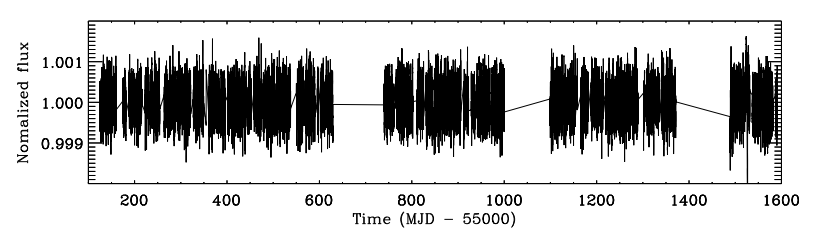
\includegraphics[width=\linewidth]{figs/reduced}
	\begin{center}
	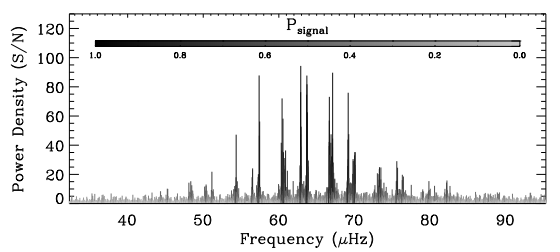
\includegraphics[width=.6\linewidth]{figs/power}
	\end{center}
	6 red giants with high S/N ratios were observed by Kepler over four years and were shown to have solar-like oscillations. Raw Kepler data was reduced and then combined into a power spectrum. 
}

\note{
	The probability here is the probabilityh that a power density is a stellar characteristic and not a part of the white noise
}

\frame{
	\frametitle{Peak-Bagging}
	Mode frequency approximation
	\begin{equation}
	\nu_{nl} \approx \Delta \nu ( n + \frac{l}{2} + \epsilon right) - \delta_{nl}
	\end{equation}
	\begin{itemize}
		\item $l$ is mode degree
		\item $n$ is radial order
		\item $\epsilon$ is stellar surface feature parameter
		\item $\delta_{nl}$ is small separation
	\end{itemize}
	In the analysis, the modes $l=0$ were determined to be radial nodes and $l=1, 2$ were most p-like and $l=1$ was individual mixed-mode
}
\note{
	Node fitting was done using monte-carlo simulations over the power spectra using $\chi^2$ and lorentzian distributions for the parameters.
}
\frame{
	\frametitle{Peak-Bagging Result}
	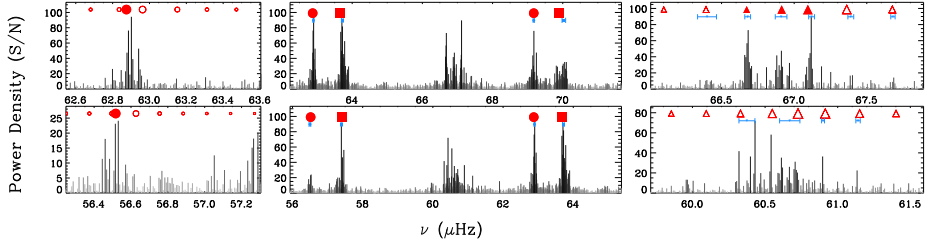
\includegraphics[width=\linewidth]{figs/peak}
	Red symbols show where certain modes would be in a best-fitting model of the spectrum. Left frame is primarily g-modes, middle is mixed modes, right is primarily p-modes.
}

\frame{
	\frametitle{Effects of Surface Correction on Wave Modes}
	\begin{center}
		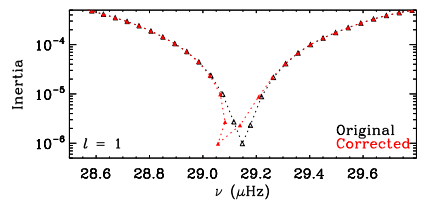
\includegraphics[width=.6\linewidth]{figs/node}
	\end{center}
	Correction for $l=1$ mixed modes due to surface parameter.
}
\frame{
	\frametitle{Surface Correction Effect}
	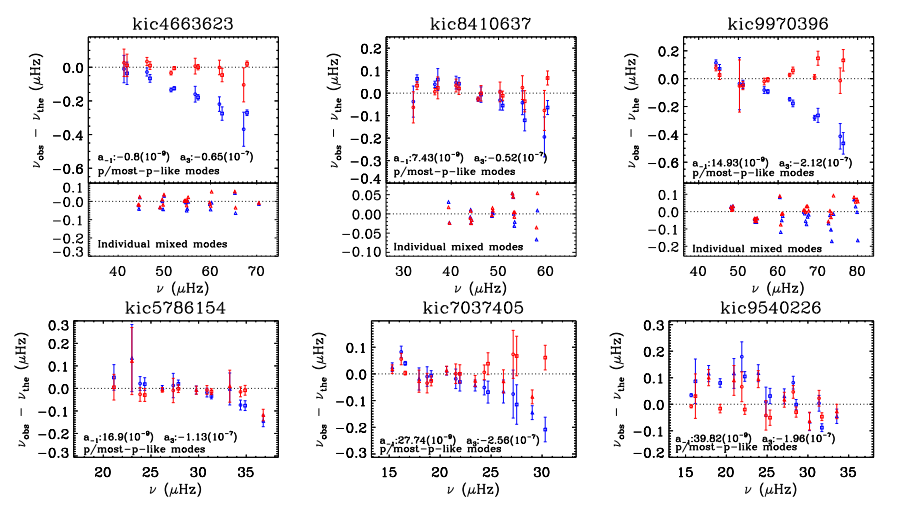
\includegraphics[width=\linewidth]{figs/change}
}
\note{
	This shows how the surface correction changed the model frequencies for each star
}

\frame{
	\frametitle{Surface Correction Correlation}
	\begin{center}
		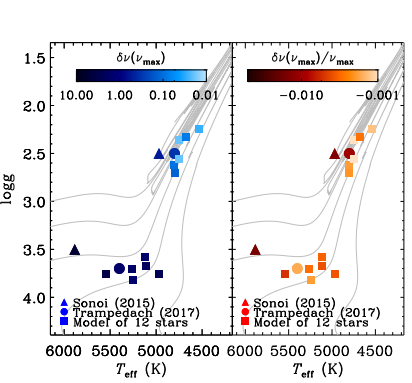
\includegraphics[width=.55\linewidth]{figs/surface}
	\end{center}
	Surface correction is dependent on surface parameters like $T_{eff}$ and $\log{g}$.
}

\frame{
	\frametitle{Surface Correction Coefficient Correlation}
	\begin{center}
		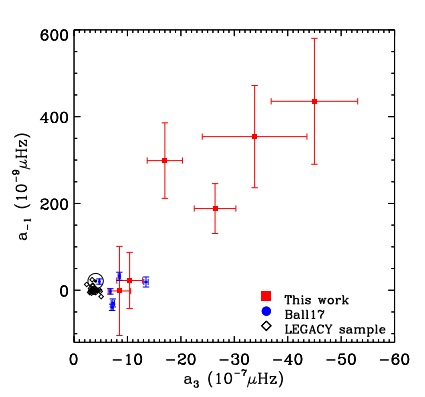
\includegraphics[width=.55\linewidth]{figs/line}
	\end{center}
	Linear correlation of $a_{-1}$ and $a_3$.
}

\frame {
	\frametitle{Stellar Models}
	MESA models:
	\begin{itemize}
		\item $ Y_0 = 0.249$
		\item $Y_{init}=Y_0+\frac{\Delta Y}{\Delta Z}Z_{init}$
		\item $X+Y+Z=1$
	\end{itemize}
	Overshoot mixing diffusion:
		$$D_{OV} = D_{conv, 0} \exp\left( {\frac{-2z}{fH_p}}\right) $$
	Surface correction:
		$$\delta_{\nu} = \frac{a_{-1} (\nu/\nu_{ac})^{-1} + a_3 (\nu/\nu_{ac})^3}{I}$$
	Acoustic cutoff:
		$$ \frac{\nu_{ac}}{\nu_{ac,\odot}}\approx\frac{g}{g_\odot} \left( \frac{T_{eff}}{T_{eff,\odot}}\right)^{-1/2} $$
}

\frame {
	\frametitle{Model Parameters Results}
	\begin{center}
	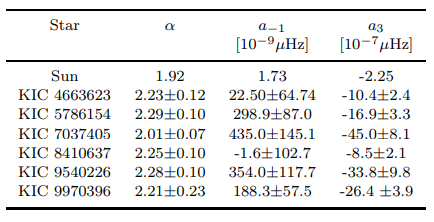
\includegraphics[width=.6\linewidth]{figs/parameters}

	\end{center}
	Model parameters were fit with a (beautiful) bayesian analysis. The parameters determined are show clearly that the mixing length parameter is larger in these red giants than the sun and that the surface correction coefficients are not solar. This mixing length is also 16\% higher than 3D hydrodynamical simulations.
}
\note{
	KIC 7037405 has different distinct results for mass and may have a higher mixing-length parameter
}


\frame {
	\frametitle{Conclusions}
	\begin{enumerate}
		\item The average mixing-length parameter of the studied red giants is \SI{1.14\pm.07} higher than calibrated solar value
		\item The calibrated mixing-length parameter is 16\% higher than the value given by 3D hydrodynamical simulations
		\item The surface wave correction term was found to affect the mixed wave modes indirectly
		\item In the studied red giants, the surface correction methods fail to fix effects in g-dominated modes
		\item The surface term correlates with $T_{eff}$, $\log{g}$ and the mixing-length parameter
		\item The coefficients in the surface correction expression increase greatly with evolution due to growth of mode inertia  
	\end{enumerate}
}

\end{document}